\documentclass{article}
\usepackage[utf8]{inputenc}

% Page setup
\usepackage[a4paper,landscape,margin=2cm]{geometry}
\usepackage{amsmath}

% Typography
\usepackage[scaled]{helvet}
\let\familydefault\sfdefault

\usepackage[usenames,svgnames]{xcolor}
\usepackage{tikz,pgfplots}
\usetikzlibrary{positioning,arrows,intersections}

%\definecolor{a}    {RGB}{199,212,104}
\definecolor{colornode} {RGB}{79 ,142,209}
\definecolor{colordict}     {RGB}{143,232,186}
\definecolor{colorhdt}      {RGB}{49 ,167,226}
\definecolor{colortext}     {RGB}{29 ,29 ,27 }

\begin{document}
\pagestyle{empty}
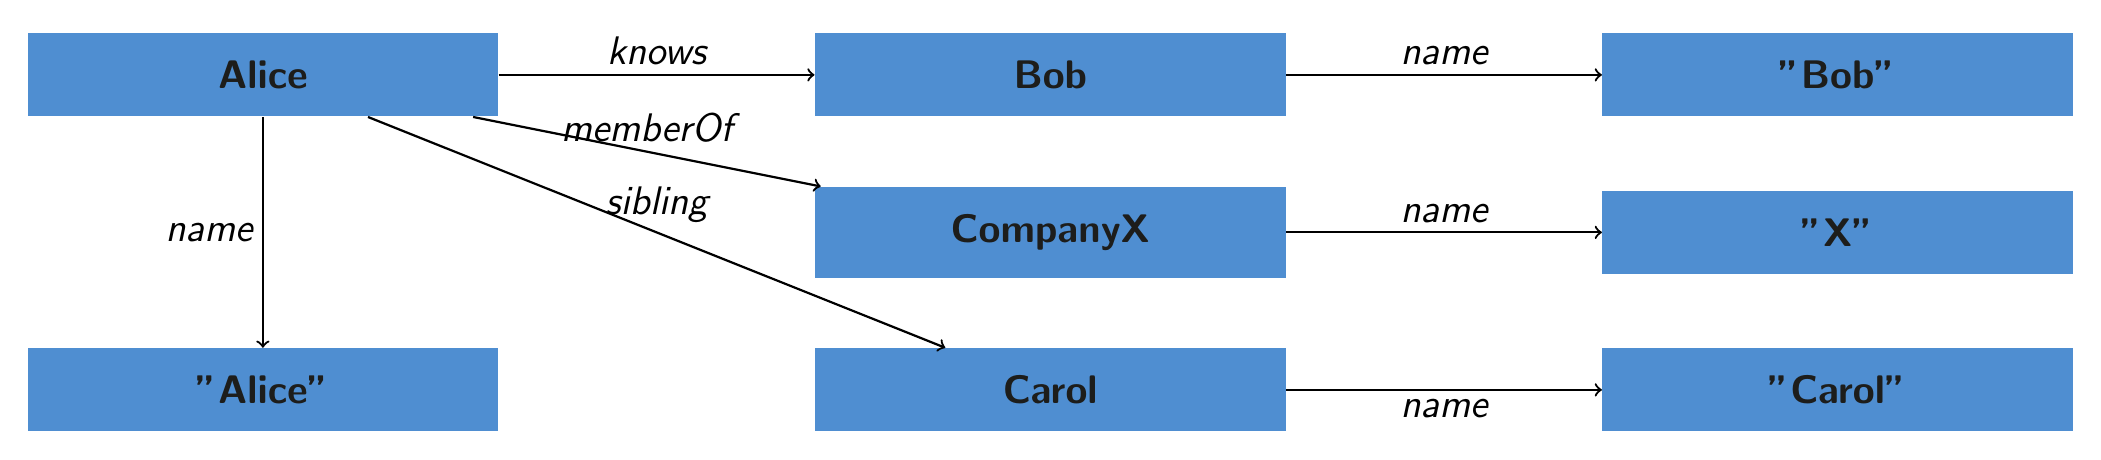
\begin{tikzpicture}[
    node distance = 2em, auto,
    font={\Large\itshape},
    base/.style={text=colortext,font={\Large\bfseries},inner sep=10pt,align=center,rectangle},
    txt/.style={text=colortext,font={\Large\bfseries},align=center},
]

    \node[base,fill=colornode,text width=15em] at (0 , 0) (alice) {Alice};
    
    \node[base,fill=colornode,text width=15em] at (0 ,-4) (name)  {"Alice"};
    \draw[->,thick](alice) -- (name) node[midway,left] {name};
    

    \node[base,fill=colornode,text width=15em] at (10,0) (bob)   {Bob};
    \draw[->,thick](alice) -- (bob)  node[midway,above] {knows};
    \node[base,fill=colornode,text width=15em] at (20,0) (bobName)   {"Bob"};
    \draw[->,thick](bob)   -- (bobName)  node[midway,above] {name};


    \node[base,fill=colornode,text width=15em] at (10,-2) (company)   {CompanyX};
    \draw[->,thick](alice) -- (company)  node[midway,above] {memberOf};
    \node[base,fill=colornode,text width=15em] at (20,-2) (companyName)   {"X"};
    \draw[->,thick](company) -- (companyName)  node[midway,above] {name};


    \node[base,fill=colornode,text width=15em] at (10,-4) (carol)   {Carol};
    \draw[->,thick](alice) -- (carol)  node[midway,above] {sibling};
    \node[base,fill=colornode,text width=15em] at (20,-4) (carolName)   {"Carol"};
    \draw[->,thick](carol) -- (carolName)  node[midway,below] {name};


\end{tikzpicture}
\end{document}
